\documentclass[12pt,preprint]{aastex}
\let\captionbox\relax
\usepackage{mathtools}
\usepackage{epstopdf}
\usepackage{amsmath}
\usepackage{graphicx}
\usepackage{caption,subcaption}
\captionsetup[figure]{labelsep=space,singlelinecheck=false}
\captionsetup[subfigure]{justification=centering}

\epstopdfDeclareGraphicsRule{.pdf}{png}{.png}{convert #1 \OutputFile}
\graphicspath{ {images/} }
\DeclareGraphicsExtensions{.png,.pdf}
\begin{document}

\title{Pushing the Limits of De-trending with PLD}

% \title{Searching for Exoplanets with Sputtering Space Telescopes}

\author{Nicholas Saunders \altaffilmark{1,2,3}, Rodrigo Luger \altaffilmark{1,2}, Rory Barnes \altaffilmark{1,2}}

\altaffiltext{1}{Department of Astronomy, University of Washington, Box 351580, Seattle, WA 98195, USA}
\altaffiltext{2}{Virtual Planetary Laboratory, Seattle, WA 98195, USA}
\altaffiltext{3}{nks1994@uw.edu}

\begin{abstract}

	As the \textit{Kepler} Space Telescope's follow-up \textit{K2} mission enters its final campaigns of observation, the fuel powering the spacecraft's stabilizing thrusters is expected to begin to run out, causing thruster fires to sputter. Sputtering will cause higher magnitude and less predictable motion of stellar Point Spread Functions (PSFs) relative to the spacecraft detector, generating more noise in transiting exoplanet light curves. To understand this increased noise, we present \texttt{skope}, a \texttt{python} package to create a forward model of the \textit{Kepler} Space Telescope detector and simulate stellar targets traversing the CCD. Using these simulations, we characterize the contribution of detector sensitivity variation to the noise of \textit{K2} light curves and test various models for thruster sputtering in preparation for identifying high motion in future \textit{K2} data. We also test methods to increase the effectiveness of existing noise-removal techniques for space telescope exoplanet targets, focusing our treatment on stars with bright neighbors or high motion relative to the detector. Using techniques tested on simulations, we study a population of exoplanet targets that has received less attention due to difficulties arising from contribution by bright nearby stars. My noise-removal methods can be applied to current and future \textit{K2} data, as well as data from future missions such as the Transiting Exoplanet Survey Satellite (\textit{TESS}) and the James Webb Space Telescope (\textit{JWST}).

\end{abstract}

\section{Introduction}

Despite the failure of two reaction wheels in 2012 and 2013, the \textit{Kepler Space Telescope} has continued to produce valuable data in its new configuration, \textit{K2}, with significantly higher precision than ground based telescopes \citep{2014PASP..126..398H}. However, due to the unstable pointing caused by the missing reaction wheels, targets have significant motion relative to the quantum sensitivity variation of the telescope detector, creating noise in \textit{K2} light curves (\textbf{source}). A number of attempts have been made to isolate and remove the instrumental noise from \textit{K2} data \citep{2015A&A...579A..19A, 0004-637X-806-1-30, 2015MNRAS.454.4159H, 2015MNRAS.447.2880A, 2016MNRAS.459.2408A}.

Existing de-trending pipelines, notably the \texttt{K2SFF} pipeline, developed by \cite{2014PASP..126..948V}, generate Gaussian fits to the stellar PSF to find the centroid position of targets. From this, motion relative to the detector can be backed out and used to de-trend \textit{K2} light curves. However, factors such as light aberration, pixel sensitivity variation, and imperfect PSF fitting can lead to uncertainty in the central pillar of these models: the motion of the star relative to the detector.

The EPIC Variability Extraction and Removal for Exoplanet Science Targets (\texttt{EVEREST}) pipeline, developed by \cite{2016AJ....152..100L, 2017arXiv170205488L} utilizes a different method -- pixel level decorrelation (PLD), developed by \cite{0004-637X-805-2-132}. PLD seeks to remove noise generated by intra-pixel sensitivity variation independent of apparent motion of the star. This method is particularly effective for \textit{K2} light curves despite the magnitude of apparent motion being high, and \texttt{EVEREST} can recover \textit{Kepler}-like accuracy in exoplanet light curves for targets up to $K_p = 15$.

There remain cases in which \textit{K2} de-trending pipelines fail to achieve \textit{Kepler}-like accuracy, particularly high magnitude stars ($K_p > 15$) and targets with bright contaminants near the edge of the aperture \citep{2017arXiv170205488L}. For PLD, this is problematic because the algorithm uses pixels containing flux from the contaminant source to de-trend the target light curve. Minimizing or removing contaminant flux from pixels included in the PLD model increases the de-trending power of \texttt{EVEREST}. Crowded apertures are not a problem unique to \textit{Kepler}/\textit{K2}, and future space telescope missions will benefit from having established methods to approach crowded targets.

Further, as the \textit{Kepler Space Telescope} runs out of fuel, its motion due to thruster fires is expected to become less predictable and the magnitude of targets' motion relative to the detector will increase. With higher motion, targets will traverse more regions of varied pixel sensitivity, contributing more noise to the light curves of \textit{K2} targets. Eventually, the telescope will enter a phase of constant drift, at which point targets will traverse many pixels across the detector and flux pollution from neighbors is likely, as stellar PSFs may overlap over the course of a campaign.

In this paper, we present options for assessing and removing these sources of noise. \S 2 and \S 3 explore the issues of pixel sensitivity variation and crowding, respectively. \S 4 describes our methods to characterize and address these sources of noise: \S 4.1 focuses on PSF-fitting, \S 4.2 on Aperture-fitting, and \S 4.3 on Motion Removal. In \S 5, we discuss our results, and finally we draw our conclusions in \S 6.

\section{Synthetic Light Curves}

\subsection{Pixel Sensitivity Variation}

Removal of instrumental noise requires a thorough understanding of its source. Stellar motion relative to the pixel sensitivity variation on the \textit{Kepler} CCD causes fluctuation in the amount of light received by the telescope detector. In order to accurately fit a PSF model to multiple targets on the detector, it became necessary to generate a model for the pixel sensitivity variation of the CCD.

We did not set out to model the exact sensitivity of the \textit{Kepler} CCD, rather our goal was to simply characterize its contribution to the noise in \textit{K2} light curves. Light curves generated against this model are adequate to serve as well-understood sample targets on which to test de-trending methods. To accurately represent the \textit{Kepler} CCD, we generated a model for the detector that included both inter-pixel sensitivity variation between pixels and intra-pixel sensitivity variation within each pixel. We found that a stochastic distribution of sensitivity with ${\sim}1\%$ variation between pixels and ${\sim}5\%$ variation within pixels, from center to edge.

A sample detector with included sensitivity variation can be seen in figure \ref{fig:detector}.

\begin{figure}[h!]
  \centering
  \begin{subfigure}[b]{0.25\textwidth}
    \centering
    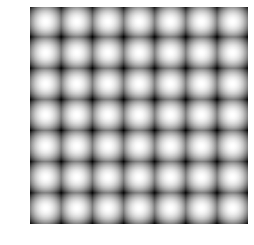
\includegraphics[width=.9\linewidth]{detector.png}
		\caption{}
  \end{subfigure}%
  \quad
  \begin{subfigure}[b]{0.25\textwidth}
    \centering
    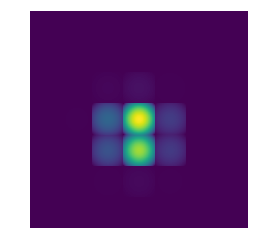
\includegraphics[width=.9\linewidth]{uninterpolated.png}
		\caption{}
  \end{subfigure}%
	\quad
	\begin{subfigure}[b]{0.25\textwidth}
		\centering
		
\includegraphics[width=.85\linewidth]{interpolated.png}
		\caption{}
	\end{subfigure}
	\caption{(a) a sample detector with sensitivity variation; (b) stellar PSF simulated onto detector; (c) interpolated image}
  \label{fig:detector}
\end{figure}

For campaigns up to 16, stellar PSFs already traverse various regions of sensitivity variation on the CCD due to pointing instability. As spacecraft motion increases, PSFs will move more dramatically across many pixels, which will contribute significant noise to sputtering-\textit{K2} light curves.

\subsection{PSF Model}

A stellar PSF was generated with a characteristic two-dimensional Gaussian shape and with covariance between $x$ and $y$ dimensions to capture PSF distortion due to incident light aberration on the \textit{Kepler} detector. We define our mathematical model to be

\[
\tag{1}
F(t)=\sum_{aperture} \iint_{pixel} [s(x)s(y)P(x,y)\tau (t)]dxdy,\\
\]

where $s(x,y)$ is the sensitivity variation function, modeled by a sum of power functions, and $P(x,y)$ is the PSF of the star, centered at $(x_0,y_0)$ with amplitude $A$. $\tau (t)$ is a simulated transit function. The pixel sensitivity model is given by

\[
\tag{2}
s(x)s(y) = \sum_n a_{x,n}x^na_{y,n}y^n \\
\]

and the PSF model is given by

\[
\tag{3}
\begin{split}
P(x,y) & = \sum_m \frac{1}{2\pi\sigma_{x,m}\sigma_{x,n}\sqrt{1-\rho_m^2}} \text{exp}\left[ -\frac{1}{2(1-\rho_m^2)} \left( \frac{(x-x_{0,m})^2}{2\sigma_{x,m}^2} \right. \right. \\
			 & \left. \left. + \frac{(y-y_{0,m})^2}{2\sigma_{y,m}^2} - \frac{2\rho_m  (x-x_{0,m})(y-y_{0,m})}{\sigma_{x,m}\sigma_{y,m}} \right) \right].
\end{split}
\]

Our model for the sensitivity variation was chosen to capture the same noise magnitude as real \textit{K2} targets. For our noise metric, we use the Combined Differential Photometric Precision, developed by the \textit{Kepler} team \citep{2012PASP..124.1279C}. In figure \ref{fig:nomotion}, we plot the CDPP of our simulated light curves with no motion against CDPP of original \textit{Kepler} light curves as a function of $K_p\ Mag$. Our synthetic targets follow the trend of photon-limited noise because our benchmark model has no stellar variability, which can add extraneous noise to de-trended light curves.

\begin{figure}[h]
	\centering
	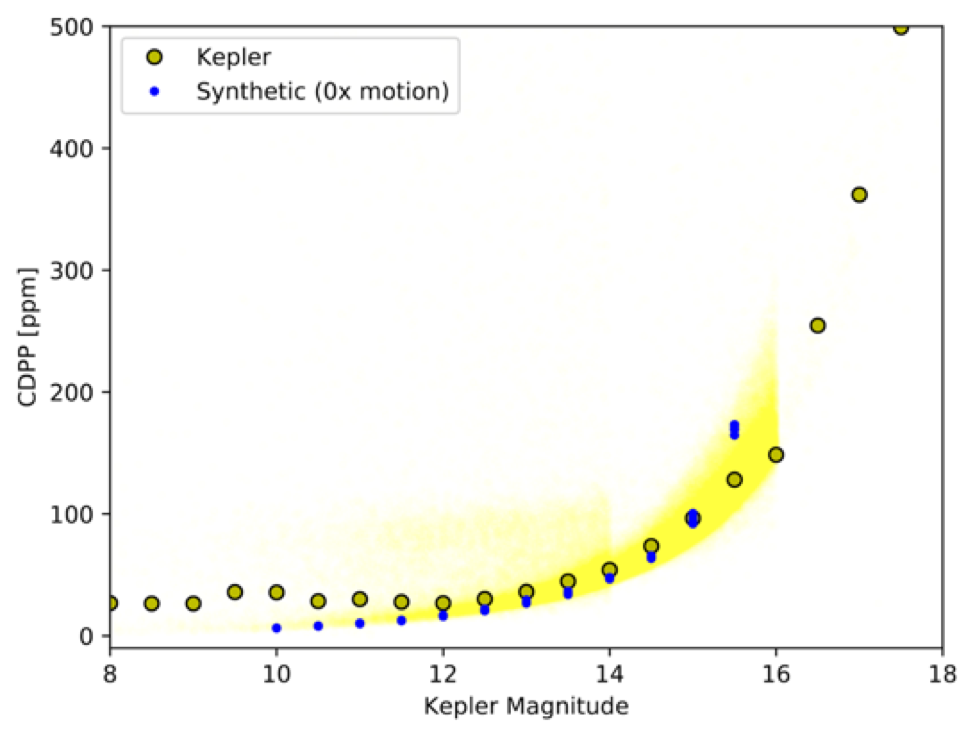
\includegraphics[width=.5\linewidth]{nomotion.png}
	\caption{CDPP of our simulated light curves with no motion compared to original \textit{Kepler} targets as a function of $K_p\ Mag$.}
	\label{fig:nomotion}
\end{figure}

In figure \ref{fig:1motion}, we inject motion from a real \textit{K2} target (EPIC 205998445) to benchmark our model against \textit{K2} data. The noise of our various tests bracket the trend of raw \textit{K2} noise, again following the photon-limited trend due to no variability.

\begin{figure}[h]
	\centering
	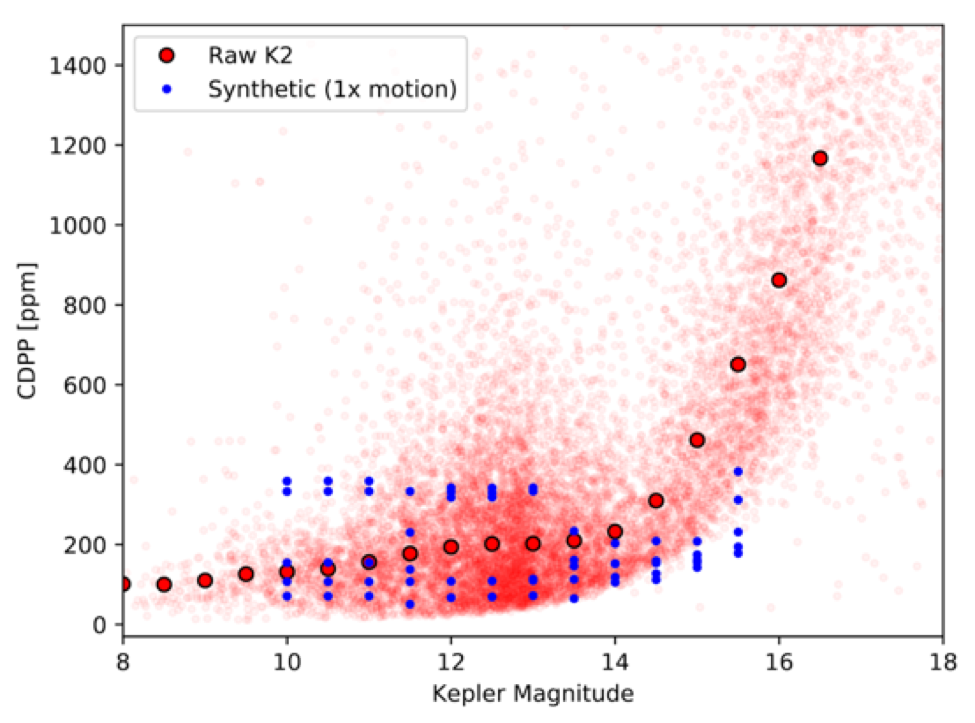
\includegraphics[width=.5\linewidth]{1xmotion.png}
	\caption{CDPP of our simulated light curves with \textit{K2} motion compared to real \textit{K2} targets as a function of $K_p\ Mag$.}
	\label{fig:1motion}
\end{figure}

The coefficients $a_n$ were determined to emulate the magnitude of sensitivity variation on the \textit{Kepler} CCD based on its contribution to the noise in \textit{K2} light curves. Sensitivity coefficients are independent in $x$ and $y$ for consistancy with \cite{toyozumi_ashley_2005}.

To best capture the characteristics of \textit{K2} data when analyzing the noise contributed by quantum sensitivity variation, our model also included two sources of noise -- synthetic photon and background noise.

This is the same model we fit to the simple aperture photometry (SAP) flux of \textit{K2} targets to subtract contaminant flux (further discussion in \S 4.1).

\subsection{Crowding}

A significant stumbling block of PLD arises when \textit{K2} targets are observed in crowded fields. In these cases, PLD uses pixels containing flux from neighbors to de-trend the target light curve, and the astrophysical signal or transit signal can be lost.

We define a crowding metric, $C$, as a quantitative measure of the significance of neighbor pollution in each pixel.

\[
\tag{4}
C = 1 - \frac{F_{target}}{F_{total}}
\]

Applications of PLD have demonstrated that it is not well suited to handle targets with high values of $C$ in pixels containing flux from the target star. These cases suffer from overfitting at a higher rate and transit recovery accuracy is compromised significantly. A sample target (EPIC 202072978) and the crowding metric $C$ for each pixel are shown in Fig. 2. This plot was achieved by simultaneously fitting PSFs to the central star and nearby contaminant, then calculating $C$ for each pixel from equation (3).

\begin{figure}[h]
	\centering
	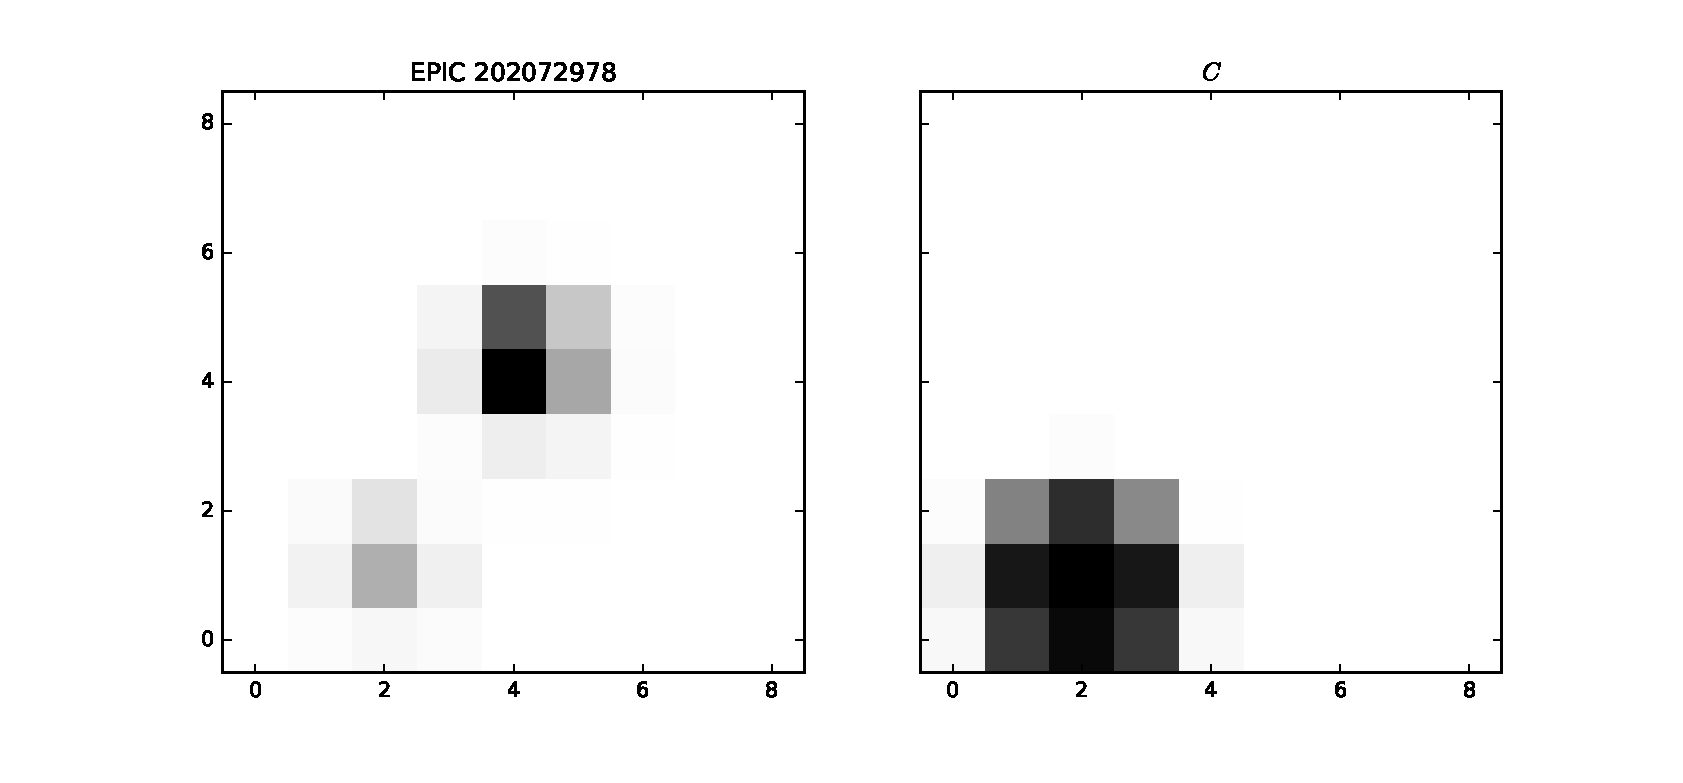
\includegraphics[width=1.0\linewidth]{cr.eps}
	\caption{A single cadence from target EPIC 202072978, a $12^{\text{th}}$ magnitude exoplanet host and its $16^{\text{th}}$ magnitude neighbor (left), and the crowding metric $C$ in each pixel for this cadence, as defined in Eq. 4 (right).}
	\label{fig:crowding}
\end{figure}

\subsection{High Roll}

To test how PLD performs on targets with high motion relative to the detector, we inject motion vectors with various coefficients into our synthetic models. A coefficient of 1 corresponds to physical \textit{K2} motion (maximum of $\sim 0.56$ pixels), while a coefficient of 20 results in motion of up to $11.2$ pixels.

\begin{table}[h!]
\begin{center}
    \begin{tabular}{c | c | c}
        Motion Coefficient & Physical Motion (pixels) & Max Motion (pixels) \\
        \hline \hline
        1 & $0.37\pm0.16$ & 0.56 \\
        2 & $0.38\pm0.32$ & 1.12 \\
				5 & $1.04\pm0.75$ & 2.8 \\
				10 & $2.04\pm1.75$ & 6.6 \\
				20 & $3.16\pm1.75$ & 11.2 \\
   \end{tabular}
	 \caption{Motion coefficients and corresponding pixel motion.}
	 \label{table:1}
\end{center}
\end{table}

The resulting raw light curve noise can be seen in Fig. \ref{fig:rawmotion} compared to raw \textit{K2} noise. Our synthetic targets with a motion coefficient of 1 align with the raw \textit{K2} trend and increase corresponding to noise coefficient.

\begin{figure}[h]
	\centering
	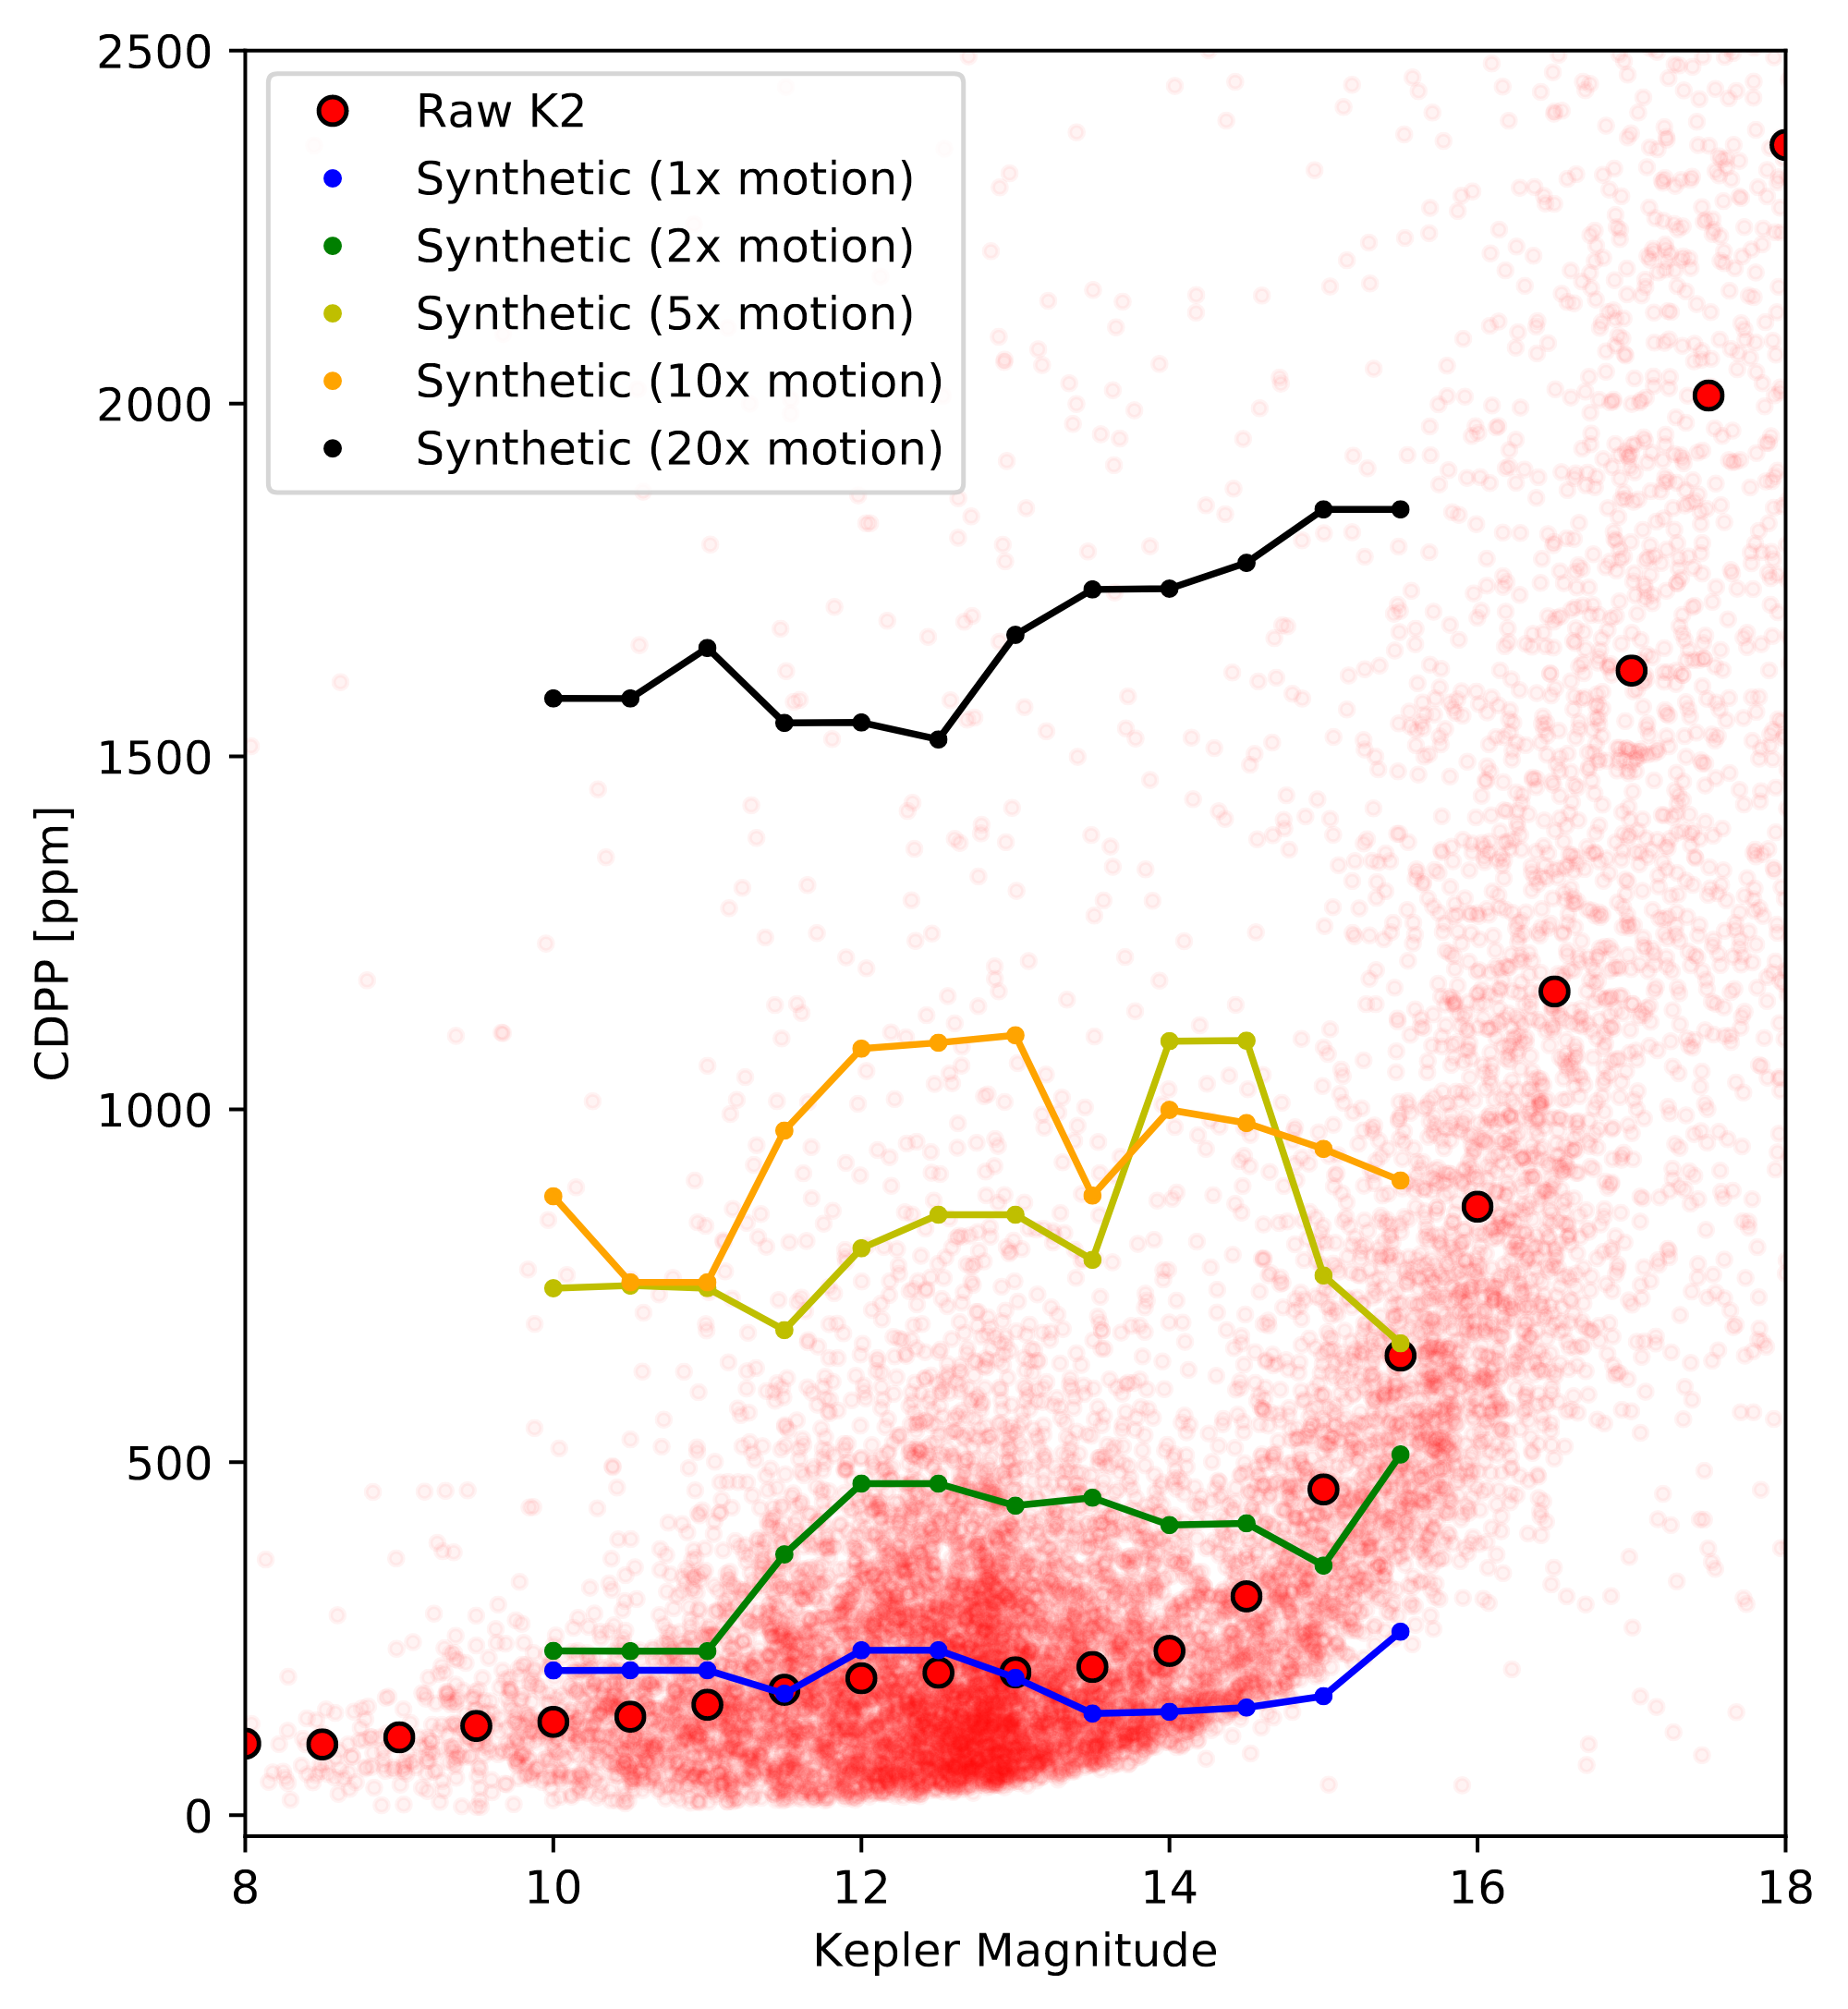
\includegraphics[width=1.0\linewidth]{rawmotion.png}
	\caption{CDPP of synthetic targets with 1x to 20x motion versus raw \textit{K2} noise as a function of $K_p\ Mag$.}
	\label{fig:rawmotion}
\end{figure}

\section{Methods}

The two sources of noise presented above -- pixel crowding and detector sensitivity variation -- have been obstacles for \textit{K2} de-trending pipelines. In the following section, we present methods to address both sources of noise and recover more accurate light curves.

\subsection{PLD}

To de-trend our synthetic light curves, we used a variant of the PLD method applied in the \texttt{EVEREST} pipeline. For a more detailed treatment of PLD, see the first two \texttt{EVEREST} papers \citep{2016AJ....152..100L,2017arXiv170205488L}. Our model included a Gaussian Process (GP) to capture and retain the astrophysical signal of the synthetic host star.

The likelihood ($\mathcal{L}$) of our model capturing the true signal of the star is captured closely by a Gaussian distribution given by

\[
\mathcal{L} = \exp{\left[-\left( \frac{\textbf{y}-\textbf{X}\cdot\textbf{w}}{2\pmb{\Sigma}} \right)^2 \right]}, \\
\]

where $\textbf{y}$ is the raw flux light curve, $\textbf{X}$ is the design matrix, $\pmb{\Sigma}$ is the covariance matrix between pixels, and $\textbf{w}$ is the array of weights. By solving for the derivative of the natural log of this likelihood, we locate the distribution peak and the best values for weights on the pixel flux vectors.

\[
\ln{\mathcal{L}} = - \frac{1}{2}\left(\textbf{y} - \textbf{X}\cdot\textbf{w} \right)^\top \cdot \pmb{\Sigma}^{-1} \cdot \left(\textbf{y} - \textbf{X}\cdot\textbf{w} \right) \\
\]

\[
\frac{d\ln{\mathcal{L}}}{d \textbf{w}} = 0 \\
\]

\[
=\frac{d}{d \textbf{w}} \left[ - \frac{1}{2} \left(\textbf{y} - \textbf{X}\cdot\textbf{w} \right)^\top \cdot \pmb{\Sigma}^{-1} \cdot \left(\textbf{y} - \textbf{X}\cdot\textbf{w} \right) \right] \\
\]

Now, we identify the ideal weights for our noise model.

\[
\textbf{w} = \left( \textbf{X}^\top \cdot \pmb{\Sigma}^{-1} \cdot \textbf{X} \right)^{-1} \cdot \textbf{X}^\top \cdot \pmb{\Sigma}^{-1} \cdot \textbf{y} \\
\]

The final model can be found by solving

\[
\textbf{m} = \textbf{X} \cdot \left( \textbf{X}^\top \cdot \pmb{\Sigma}^{-1} \cdot \textbf{X} \right)^{-1} \cdot \textbf{X}^\top \cdot \pmb{\Sigma}^{-1} \cdot \textbf{y}. \\
\]

\subsection{PSF-fitting}

For some targets, particularly those with exceptionally close neighbors, defining an aperture around the central star can be difficult, because pixels containing flux pollution also contain important stellar signal. Exclusion of pixels above the prescribed crowding cutoff would render the remaining flux inadequate to thoroughly analyze transiting exoplanet targets.

We present a second method to remove unwanted neighbor signal: fitting each target in the frame with a Gaussian PSF model and subtracting the flux contributed by the neighbor from each pixel. This process involves constructing sums of $n$ PSFs, where $n$ is the number of stars within the aperture, and minimizing $\chi^2$ between the model, $m$ and flux, $y$. $\chi^2$ is given by

\[
\tag{5}
\chi^2 = \left( \frac{m-y}{\sigma} \right)^2,
\]

Where $\sigma$ is the flux error. Our model, defined in equation (2), was fit to each cadence of crowded \textit{K2} targets.

\subsection{Aperture-fitting}

The simplest solution to the issue of crowded apertures is to only consider pixels that contain the most flux from the desired target and exclude flux received by neighboring stars. The crowding metric in each pixel can be used to determine which pixels should be included to maximize target flux. (\textit{I need to give this a more thorough treatment to determine exactly what value of $C$ is best to include within an aperture. To do so, I will perform aperture tests on a variety of targets and maximize injected transit recovery accuracy to constrain ideal values of $C$.}) In a process we refer to as aperture PLD (aPLD), we define an aperture based on the crowding metric in each pixel to maximize target flux.

Injection tests were performed by removing noise from simulated light curves with aPLD and measuring the transit depth of the de-trended light curve. Comparing this value to the injected depth, we determine the effectiveness of aPLD and constrain useful values of $C$. With our injection tests, we find that pixels with $C>0.3$ should be excluded to maximize the effectiveness of aPLD.

\section{Results}

\subsection{Motion Tests}

When de-trended with second order PLD, our synthetic light curves align with the noise of original \textit{Kepler} observations for motion coefficients of 1x, 2x, and 5x. 10x motion shows increased noise in the de-trended light curve, but still performs better than observations from the ground.

\begin{figure}[h]
	\centering
	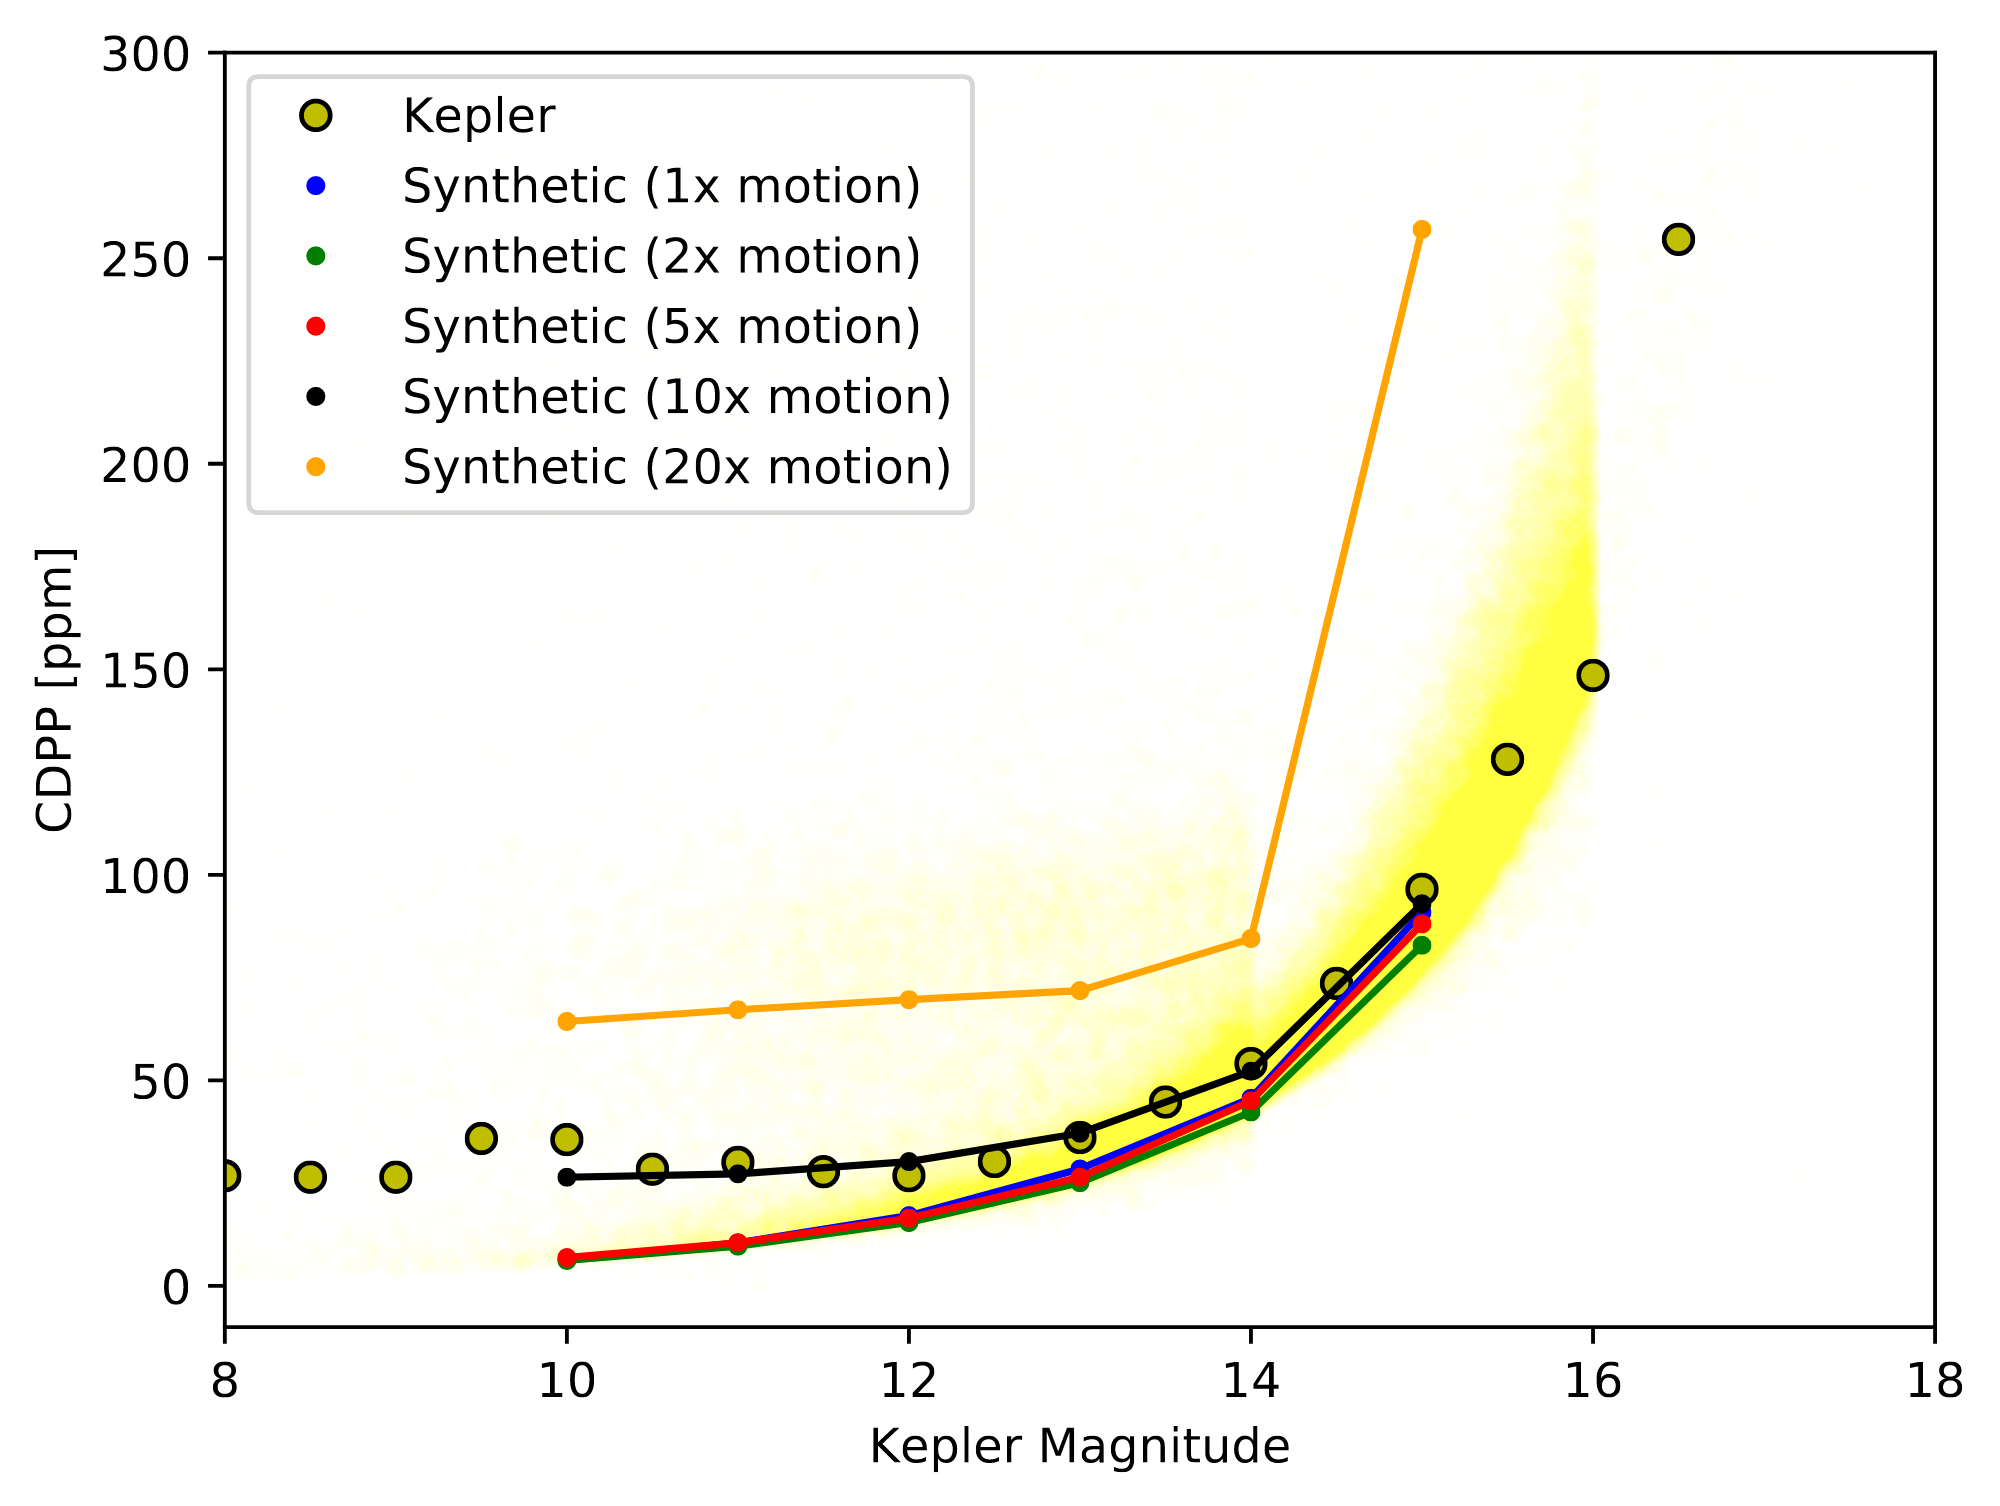
\includegraphics[width=1.0\linewidth]{detmotion.png}
	\caption{De-trended CDPP for synthetic targets with 1x to 20x motion versus original \textit{Kepler} noise as a function of $K_p\ Mag$.}
	\label{fig:detmotion}
\end{figure}

\subsection{Injection Tests}

\section{Further Considerations}

\subsection{Focus Changes}

When \textit{TESS} launches, it will begin observation with a known focusing issue, resulting in larger stellar PSFs. Further, the space telescope's trajectory will cause a periodic variation in the incident sunlight on the telescope, which will affect the quantum sensitivity of pixels. Changing sensitivity will cause \textit{TESS} PSFs to ``breathe'' as the temperature rises and falls, and apertures around \textit{TESS} targets will need to breathe correspondingly.

\subsection{Seeing}

\textbf{Not sure about this stuff yet.}

These methods can also be applied to ground-based observations. PSF aberration due to seeing contributes significant noise to observations which can be identified and removed by PLD. \textbf{Talk to Brett, use APO data.}

\section{Conclusion}

\clearpage
\bibliographystyle{aasjournal}
\bibliography{references.bib}

\end{document}
